\section{Materials and methods}

% En estos capítulos, es necesario describir:
% •	los aspectos más relevantes del diseño y desarrollo del trabajo
% •	la metodología elegida para realizar este desarrollo, describiendo las alternativas posibles, las decisiones tomadas, y los criterios utilizados para tomar estas decisiones.
% •	descripción de los productos obtenidos.
 
% La estructuración de los capítulos puede variar en función del tipo de trabajo.  
 
% En caso de que proceda, se incluirá un apartado de “Valoración económica del trabajo”. Este apartado indicará los gastos asociados al desarrollo y mantenimiento del trabajo, así como los beneficios económicos obtenidos y un análisis final sobre la viabilidad del producto.

\subsection{Data Acquisition}

\subsubsection{Mouse MSI-1 and MSI-1's RMM1}

\href{https://www.uniprot.org/}{\texttt{Uniprot}'s database} was consulted for the structure of the mouse MSI-1 protein (see \textbf{Figure \ref{fig:Q61474uniprot}}). Unfortunately, there was no NMR crystal structure for the complete protein: the only available complete structure was \texttt{AlphaFold}'s prediction of the structure (see \textbf{Figure \ref{fig:3DMSI}}). Said structure had low confidence in the aminoacid sequence not corresponding to the RRMs. Therefore, the crystal structure of MSI-1's RRM1 (see \textbf{Figure \ref{fig:3DRRM1}}) was to be employed instead for the docking simulations.

\begin{figure}[htbp!]
    \centering
    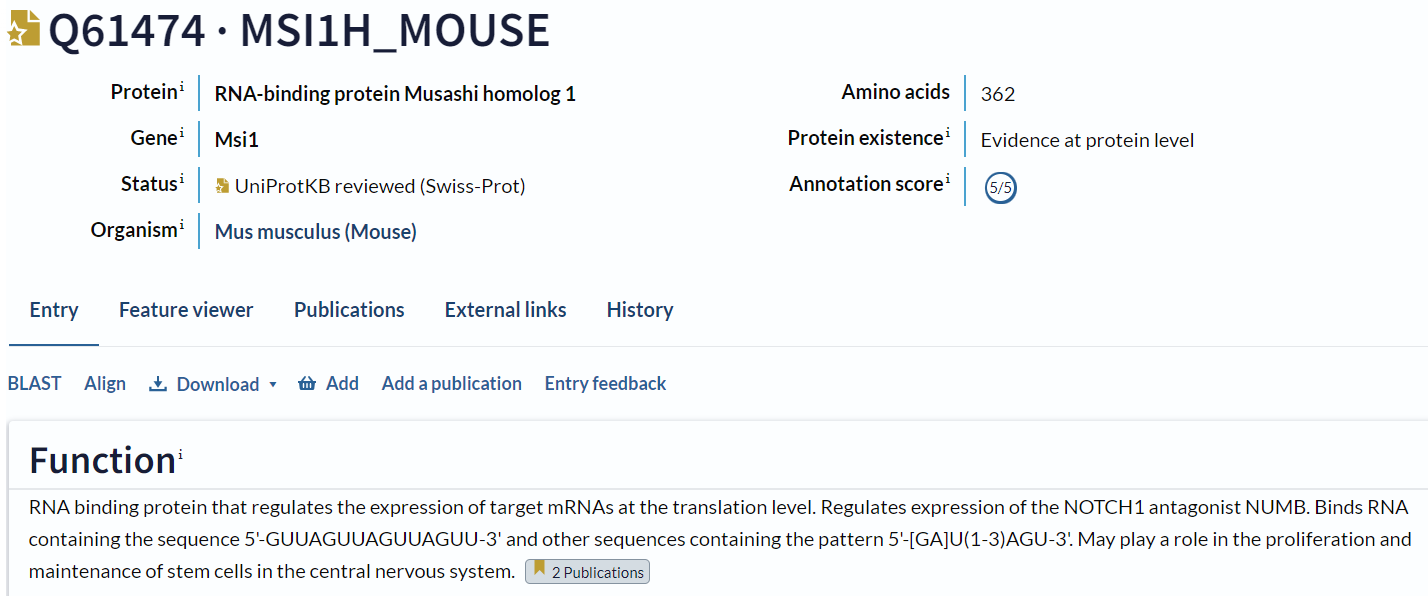
\includegraphics[width=\linewidth]{assets/Q61474_uniprot_entry.png}
    \caption[\href{https://www.uniprot.org/uniprotkb/Q61474/entry}{Uniprot entry Q61474} corresponding to the mouse MSI-1.]{\href{https://www.uniprot.org/uniprotkb/Q61474/entry}{Uniprot entry Q61474} corresponding to the mouse MSI-1 (as seen on 08/01/2023).}
    \label{fig:Q61474uniprot}
\end{figure}

The crystal NMR structure was downloaded as a \texttt{.pdb} file.

\subsubsection{Fatty acids}

The fatty acids to be employed down the line in the docking simulations were retrieved from their respective \href{https://www.chemspider.com/}{\texttt{Chemspider}} entries. The fatty acids downloaded were:

\begin{itemize}
    \item\href{https://www.chemspider.com/Chemical-Structure.392692.html}{arachidonic acid}
    \item\href{https://www.chemspider.com/Chemical-Structure.4444105.html}{linoleic acid}
    \item\href{https://www.chemspider.com/Chemical-Structure.393217.html}{oleic acid}
    \item\href{https://www.chemspider.com/Chemical-Structure.960.html}{palmitic acid}
    \item\href{https://www.chemspider.com/Chemical-Structure.5091.html}{stearic acid}
\end{itemize}

The molecules are shown in \textbf{Figure \ref{fig:fatty_acids}}.

\begin{figure}[htbp!]
    \centering
    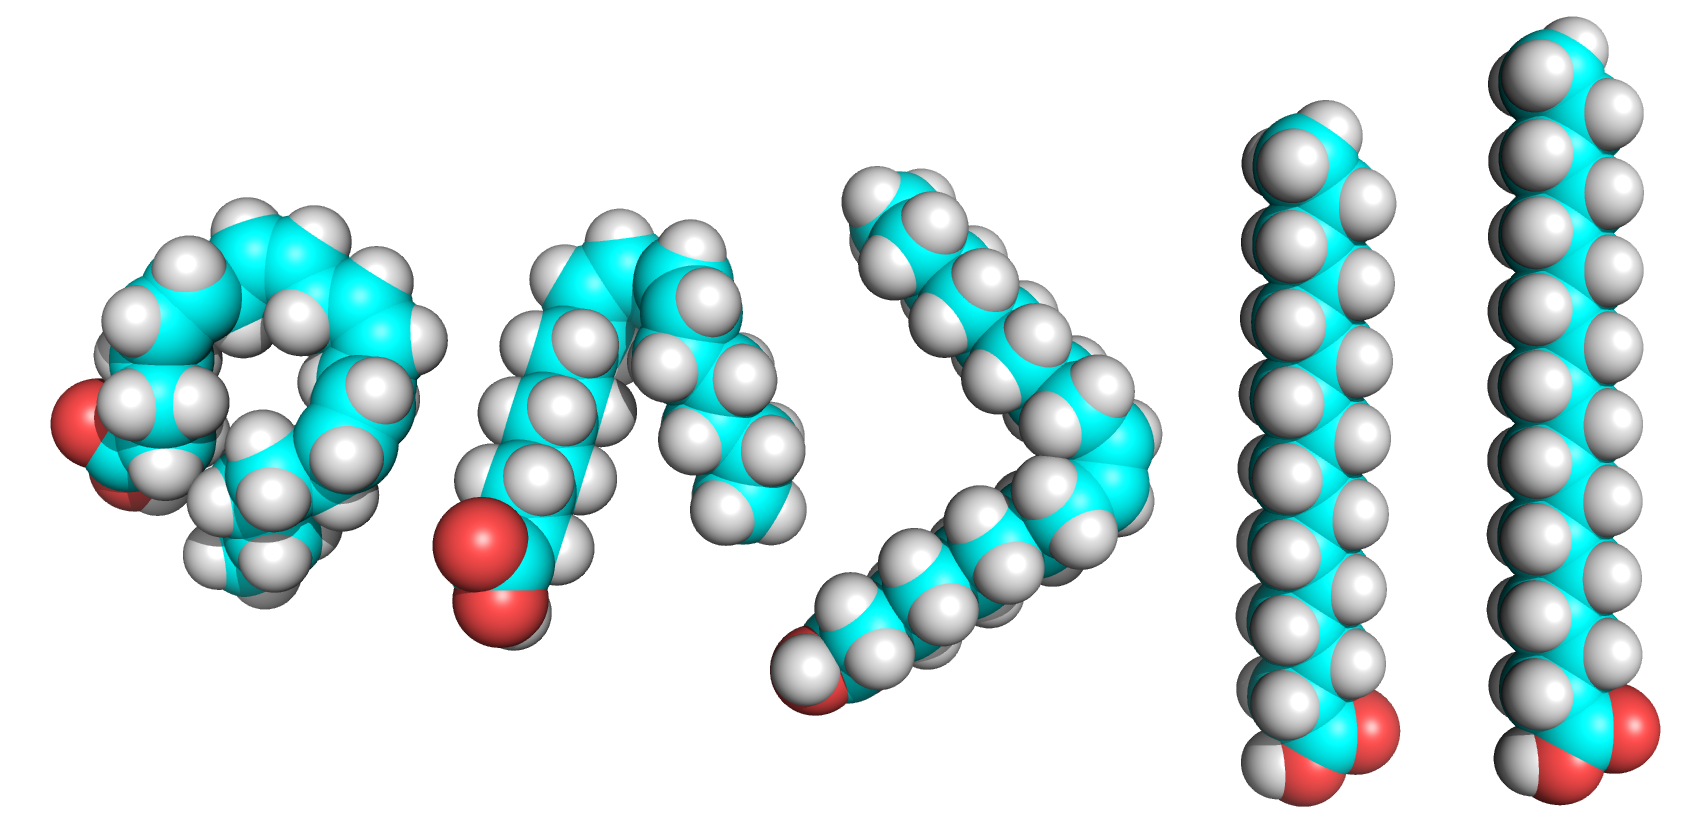
\includegraphics[width=0.75\linewidth]{assets/fatty_acids.png}
    \caption[3D structure of the fatty acids to be employed.]{3D structure of the fatty acids to be employed. From left to right: arachidonic acid, linoleic acid, oleic acid, palmitic acid and stearic acid. Colors represent the atoms present in the structures: cyan is Carbon, red is Oxygen and white is Hydrogen. Visualized through \href{https://pymol.org/2/}{\texttt{Pymol}}.}
    \label{fig:fatty_acids}
\end{figure}

The molecules' 3D structures were downloaded as \texttt{.mol} files. 

\subsection{Generation of 3D RNA molecule structures}

The raw RNA sequences to be employed were retrieved from \cite{dolcemascolo_2022} and are shown in \textbf{\nameref{appendix_A}}, where they crafted small RNA oligos based on a the selex optimal RNA sequence. RNA takes specific spatial conformations when in aqueous media, be it \textit{in vitro} or \textit{in vivo}, which can be computed directly from the RNA sequence by means of pre-measured experimental parameters \cite{santalucia_1998}.\\

To do so, the Nupack software was employed \cite{dirks_2004} (specifically its associated \texttt{Python} package) and the structures in dot-bracket notation\footnote{Dot-bracket notation is a simplistic manner of representing DNA or RNA secondary structure. For more details, see \cite{rna_structure_notations}.} were recorded. In addition, the sequences were subjected to pairwise alignments (by means of MAFFT \cite{katoh_2002}) to highlight the mutations present with respect to the original oligo. The \texttt{Python} script employed to perform these computations is found in \textbf{\nameref{appendix_B}}.

\vfill

\pagebreak

The results are shown in \textbf{Figure \ref{fig:dataset}}:

\begin{figure}[htbp!]
    \lstinputlisting[basicstyle=\tiny]{assets/dataset.tsv}
    \caption{RNA sequences along with the result of the pairwise alingments and Nupack's prediction of their secondary structure.}
    \label{fig:dataset}
\end{figure}

With this information (RNA sequence and secondary structure), the 3D conformation of each of the RNA motifs was computed by means of the \href{https://rnacomposer.cs.put.poznan.pl/}{\texttt{RNAComposer}} web server \cite{biesiada_2016} and downloaded in \texttt{.pdb} format. The corresponding 3D structures of the RNA motifs are shown in \textbf{Figure \ref{fig:RNAs}}.

\begin{figure}[htbp!]
    \centering
    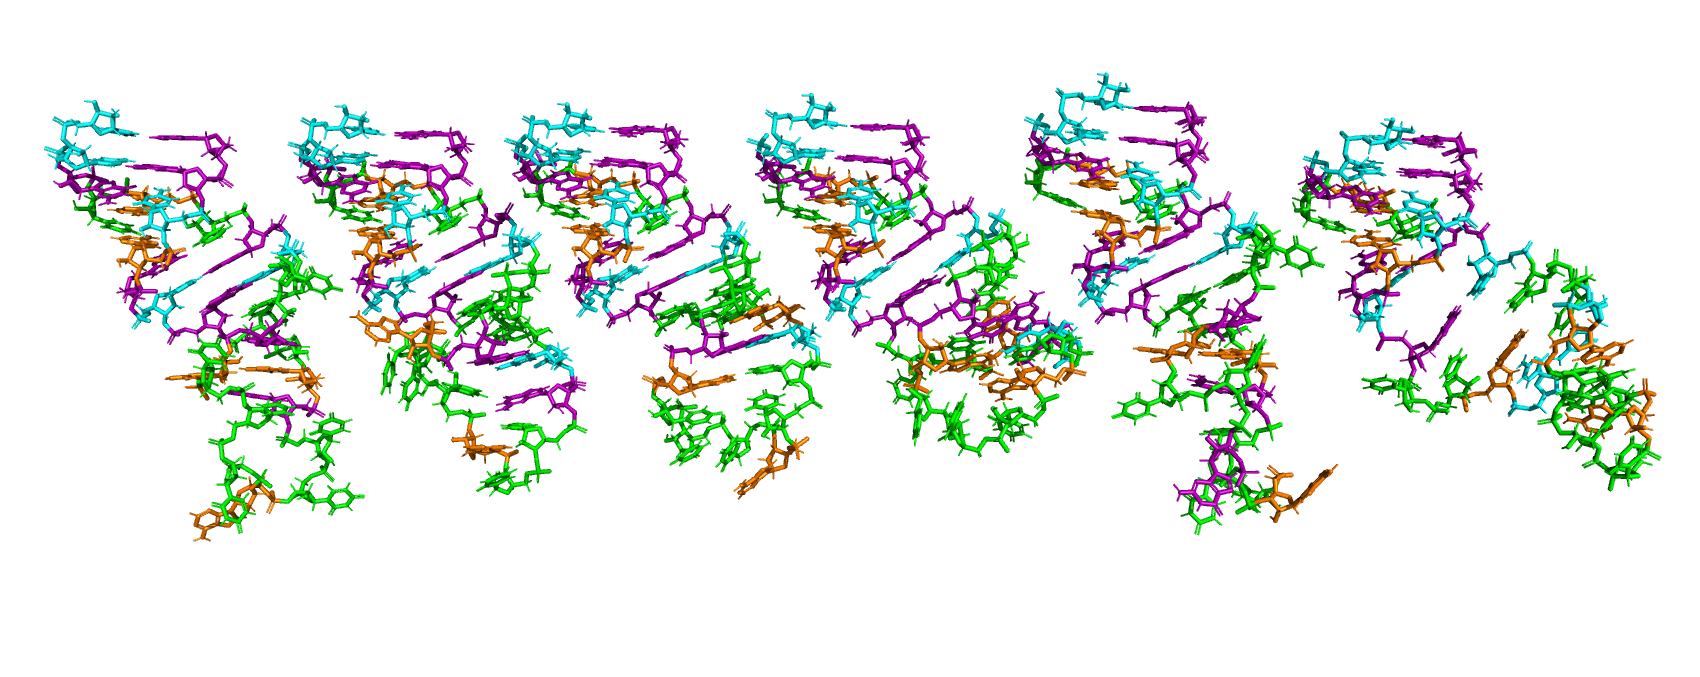
\includegraphics[width=\linewidth]{assets/RNAs.png}
    \caption[3D structures of the RNA motifs.]{3D structures of the RNA motifs. From left to right: the original RNA motif followed by the 5 mutants. Colors represent the nucleotidic bases: orange is Adenine, purple is Guanine, cyan is Cytosine and green is Uracil. Visualized through \href{https://pymol.org/2/}{\texttt{Pymol}}.}
    \label{fig:RNAs}
\end{figure}

With the 3D structures of the RNA motifs, the next step is to prepare the protein-RNA docking simulations.

\subsection{Protein-RNA docking simulations with \texttt{LightDock}}

For the protein-RNA docking simulations, the \texttt{LightDock} \cite{jimenez_garcia_2017} docking software was chosen. The main reasons are the simplicity of \texttt{LightDock}, the quality of the documentation and that the software is written in \texttt{Python}, which eases debugging steps in case of complications. Originally, \texttt{LightDock} was not meant for protein-RNA docking simulations. However, by means of some reasearch and auxiliary \texttt{Python} scripts, a simple and novel pipeline was designed which makes it possible to perform such docking simulations with \texttt{LightDock}. This pipeline takes inspiration on the \href{https://lightdock.org/tutorials/0.9.3/dna_docking}{protein-DNA docking example tutorial from the \texttt{LightDock} documentation}.

\subsubsection{Protein preparation}

First, MSI-1's RRM1 \texttt{.pdb} file needs to have their hydrogen atoms modified and relabeled so that they match the \texttt{AMBER94} force field, which is the parameter set that is going to be used in this docking simulation. To do so, the softwares \href{https://github.com/rlabduke/reduce}{\texttt{REDUCE}} and \href{https://github.com/haddocking/pdb-tools/}{\texttt{PDB-Tools}} \cite{rodrigues_2018} were employed.\\

In addition, the MSI-1's RRM1 \texttt{.pdb} file needed an additional motification related to the \texttt{AMBER94} force field: regular \texttt{.pdb} files employ the \texttt{HIS} identifier for the histidine aminoacid, which does not appear in the \texttt{AMBER94} force field. The reason behind this is that for the \texttt{AMBER94} force field, histidine can be one of 3 possible residues \cite{amber_histidine}:

\begin{enumerate}
    \item\texttt{HID}: histidine with a single hydrogen on the delta nitrogen
    \item\texttt{HIE}: histidine with a single hydrogen on the epsilon nitrogen
    \item\texttt{HIP}: histidine with hydrogens on both nitrogens (delta and epsilon). This histidine has a positive charge
\end{enumerate}

Therefore, one has to check which kind of histidine residue is present in the molecule, and change it for the corresponding \texttt{AMBER94}-compatible identifier. This can be done with a simple \texttt{Python} script called \texttt{fixHIS}, which is found in \textbf{\nameref{appendix_C}}.

\subsubsection{RNA preparation}

Similar to the protein, the RNA structures' \texttt{.pdb} file need to have their hydrogen atoms modified and relabeled. Again, the softwares \href{https://github.com/rlabduke/reduce}{\texttt{REDUCE}} and \href{https://github.com/haddocking/pdb-tools/}{\texttt{PDB-Tools}} \cite{rodrigues_2018} were employed.\\

In addition, \texttt{REDUCE} adds the 3' and 5' hydroxile groups to the RNA structures. These atoms aren't present in the \texttt{AMBER94} force field, therefore it is mandatory to remove them in order to avoid issues downstream. This can be done with a simple \texttt{Python} script called \texttt{removeEnds.py}, which is found in \textbf{\nameref{appendix_D}}.\\

Next, due to particularities of \texttt{REDUCE} for nucleic acids, it is necessary to rename and remove incompatible atom types present in the RNA structure. Again, this can be done with a simple \texttt{Python} script called \texttt{reduce\_to\_amber.py}, which is found in \textbf{\nameref{appendix_E}}. Note that the aforementioned \texttt{Python} script is an adaptation of the original version provided in the \href{https://lightdock.org/tutorials/0.9.3/dna_docking}{protein-DNA docking example tutorial from the \texttt{LightDock} documentation}.\\

Finally, in order to sucessfully run \texttt{LightDock}'s setup phase, it is mandatory to remove the \texttt{R} tags within the RNA structures. The \texttt{R} tags are important because they indicate which \texttt{AMBER94} parameters to use during the docking simulations, however one of \texttt{LightDock}'s dependencies in the setup phase (\href{http://prody.csb.pitt.edu/}{\texttt{ProDy}}) has conflicts with this notation. This removal can be done with a simple \texttt{Python} script called \texttt{manipulateRNA.py}, which is found in \textbf{\nameref{appendix_F}}.

\subsubsection{\texttt{LightDock} setup and simulation}

\texttt{LightDock}'s setup itself is simple, as it only consists of executing the setup script with the structures prepared in the previous steps, as shown in \textbf{Figure \ref{fig:lightdocksetup}}:

\begin{figure}[htbp!]
    \lstinputlisting[language=bash]{assets/lightdocksetup.sh}
    \caption{\texttt{LightDock} setup command.}
    \label{fig:lightdocksetup}
\end{figure}

The setup will generate, among other files, the simulation-ready structures\linebreak \texttt{lightdock\_protein.pdb} and \texttt{lightdock\_rna.pdb}. For the docking simulation to be successful, it is crucial to add the \texttt{R} tags within the \texttt{lightdock\_rna.pdb} RNA structure, which is basically reversing the tag removal process performed earlier. This can be achieved with a simple \texttt{Python} script called \texttt{manipulateRNAagain.py}, which is found in \textbf{\nameref{appendix_G}}.\\

\subsubsection{\texttt{LightDock} docking simulation, clustering and ranking}

If the previous steps executed without issues, it is possible to run \texttt{LightDock} as shown in \textbf{Figure \ref{fig:lightdockexec}}:

\begin{figure}[htbp!]
    \lstinputlisting[language=bash]{assets/lightdockexec.sh}
    \caption[\texttt{LightDock} execution command.]{\texttt{LightDock} execution command, using the \texttt{DNA} scoring function for nucleic acids and 4 processing cores.}
    \label{fig:lightdockexec}
\end{figure}

Once the simulation ends, and in order to be able to do the clustering and ranking step, it is mandatory to remove the \texttt{R} tags added to \texttt{lightdock\_rna.pdb} for the simulation step. For that, once again the script \texttt{manipulateRNA.py} shown in \textbf{\nameref{appendix_F}} is employed.\\

Next, the clustering and ranking can be performed in the same way as specified in the \href{https://lightdock.org/tutorials/0.9.3/dna_docking}{protein-DNA docking example tutorial from the \texttt{LightDock} documentation}. The \texttt{bash} script performing the ranking and clustering steps is shown in \textbf{\nameref{appendix_H}}.\\

The ranking will generate a \texttt{solutions.list} file where the different models generated by \texttt{LightDock} are scored. For this work, the top 10 best scoring models were taken.\\

The entire pipeline followed in this section has been implemented as a \texttt{bash} script called \texttt{run1.sh}, which is found in \textbf{\nameref{appendix_I}}. Given a\linebreak\texttt{target\_protein.pdb} file and a \texttt{ligand\_rna.pdb} file, \texttt{run1.sh} is executed as shown in \textbf{Figure \ref{fig:execrun1}}:

\begin{figure}[htbp!]
    \lstinputlisting[language=bash]{assets/run1exec.sh}
    \caption[Execution of the \texttt{run1.sh} script.]{Execution of the \texttt{run1.sh} script.}
    \label{fig:execrun1}
\end{figure}

A refined version of this pipeline has been contributed to the \href{https://lightdock.org/tutorials/0.9.3/index.html}{official \texttt{LightDock} tutorials section}. In said version, the \texttt{Python} scripts for file manipulation have been cleaned-up and applied to model the \href{https://www.rcsb.org/structure/1a1t}{1A1T protein-RNA complex}. This tutorial can be directly accessed \href{https://lightdock.org/tutorials/0.9.3/rna_docking}{here}.

\subsection{Lipid-protein docking simulations with \texttt{AutoDock Vina}}

For the lipid-protein docking simulations, \texttt{AutoDock Vina} docking software was employed. The main reasons for changing the docking software at this step are that for now \texttt{LightDock} does not feature full support of lipid-protein docking and that \texttt{AutoDock Vina} is license free. For the preparation steps, the \texttt{AutoDock Tools} is used for simplicity, although other software could have been used instead.

\subsubsection{Protein preparation}

First, MSI-1's RRM1 \texttt{.pdb} is loaded into \texttt{AutoDock Tools}, which displays all the models present in said file, as show in \textbf{Figure \ref{fig:autodockprotein}}:

\begin{figure}[htbp!]
    \centering
    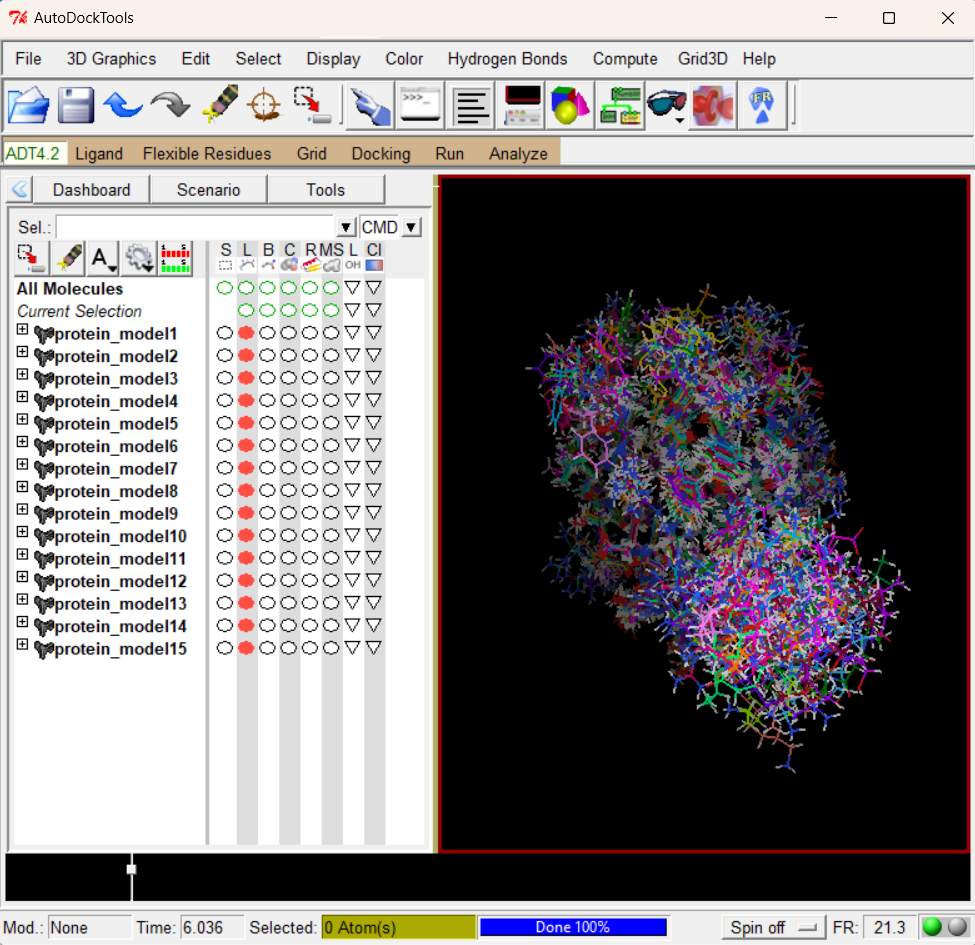
\includegraphics[width=0.8\linewidth]{assets/AutoDockTools_load_protein.png}
    \caption{Protein models in \texttt{AutoDock Tools}.}
    \label{fig:autodockprotein}
\end{figure}

It is mandatory to discard the models that are not going to be used in the docking simulations. For simplicity, in this work the model to be kept is the first one.\\

Next, there are a series of procedures to prepare the protein model for docking:

\begin{enumerate}
    \item Remove the water molecules by clicking \texttt{Edit>Delete Water}. This step may be skipped if there are no water molecules present.
    \item Add polar hydrogen atoms by clicking \texttt{Edit>Hydrogens>Add} and then select \texttt{Polar Only}. Again, this step may be skipped if the hydrogen atoms are already present.
    \item Add Kollmann charges by clicking \texttt{Edit>Charges>Add Kollmann Charges}. This step is unskippable and it is essential for the docking simulation to be successful.
\end{enumerate}

Once these steps are completed, the protein model is ready for docking and can be saved in \texttt{.pdbqt} format by clicking \texttt{Grid>Macromolecule>Choose...}.

\subsubsection{Lipid preparation}

The fatty acid molecules also need a preparation step prior to the docking simulation. First, it is necessary to convert the fatty acid models from \texttt{.mol} format to \texttt{.pdb} format. One way to do this is to open the \texttt{.mol} file in \href{https://pymol.org/2/}{\texttt{Pymol}} and then saving it in \texttt{.pdb} format. An alternative way would be to use an online file converter, such as \href{https://datascience.unm.edu/tomcat/biocomp/convert}{this one}.\\

Next, the fatty acid in \texttt{.pdb} format is loaded into \texttt{AutoDock Tools}, where preparation is done by clicking \texttt{Ligand>Input>Choose...} and selecting the fatty acid by clicking \texttt{Select Molecule for AutoDock4}. This will remove hydrogens and compute charges, which renders the fatty acid ready for codking. The model is then exported by clicking \texttt{Ligand>Output>Save}.

\subsubsection{Grid preparation}

One requirement for running \texttt{AutoDock Vina} is knowing the ``pocket'' which the ligand molecule interacts with. This site is specified by a hexahedron that delimits the spatial area where this site resides (i.e. a grid box), as shown in \textbf{Figure \ref{fig:gridbox}}.\\

If the binding ``pocket'' is unknown, the grid box can be made big so that several conformations around the protein are explored. In the case of MSI-1's RRM1, the binding pocket that interacts with the fatty acids was described in detail by Clingman and colleagues \cite{clingman_2014}, and can be seen easily in the rightmost protein of \textbf{Figure \ref{fig:3DRRM1}}.\\

With this information, the grid box was manually restrained and exported by clicking \texttt{File>Output grid dimensions file}. The grid dimensions file can be found in \textbf{\nameref{appendix_J}}. The selected grid box will be remain the same for all the protein-lipid docking simulations, because the target protein (MSI-1's RRM1) will remain unchanged.

\begin{figure}[htbp!]
    \centering
    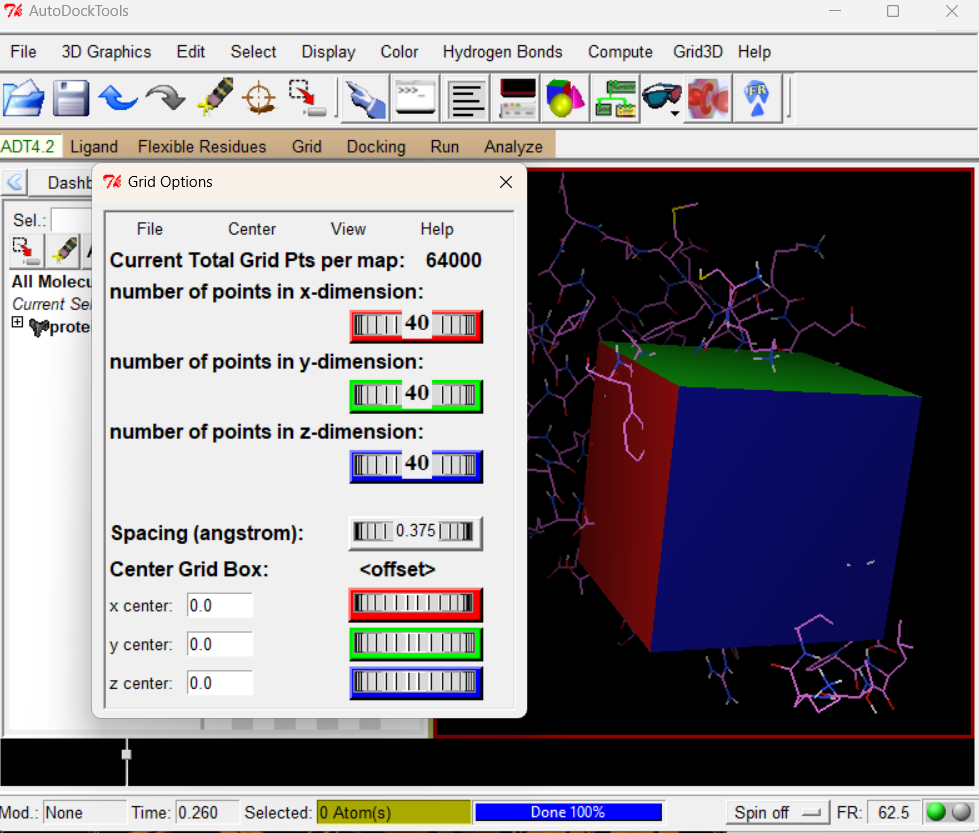
\includegraphics[width=0.8\linewidth]{assets/AutoDockTools_BOX.png}
    \caption{\texttt{AutoDock Tools} generic grid box.}
    \label{fig:gridbox}    
\end{figure}

Next, the config file for \texttt{AutoDock Vina} has to be created. This file must contain the protein model name, the ligand model name, the information found in the grid file and two additional parameters: energy range and exhaustiveness. For the latter two parameters, which control the energy spread between the best and the worst output models and the number of times the simulation is executed respectively, the default parameters \texttt{range = 4} and \texttt{exhaustiveness = 8} are employed. The config file to be used in the protein-lipid docking simulations can be found in \textbf{\nameref{appendix_K}}.\\

The following step is to run the docking simulation itself.

\subsubsection{\texttt{AutoDock Vina} simulation}

Running a docking simulation with \texttt{AutoDock Vina} requires the prepared protein model in \texttt{.pdbqt} format, the preared ligand model in \texttt{.pdbqt} format and an appropriate config file. Then, a simulation is run with the command show in \textbf{Figure \ref{fig:execvina}}:

\begin{figure}[htbp!]
    \lstinputlisting[language=Bash]{assets/runVina.sh}
    \caption{Execution of a docking simulation with \texttt{AutoDock Vina}.}
    \label{fig:execvina}
\end{figure}

The file \texttt{output.pdb} contains the result of the docking simulation and consists of the ligand molecule in 9 different conformations. The log file contains information related to the run and the energy scores of each of the conformations. The visualization of the docking simulation result is done by loading the protein model and the \texttt{output.pdb} file simultaneously in a software such as \href{https://pymol.org/2/}{\texttt{Pymol}}.

\subsection{Lipid-protein-RNA complex visualization}

The visualization of the lipid-protein-RNA is done by manually aligning the models of the protein-RNA docking simulations with the models of the protein-lipid docking simulations. This procedure is not conceptually optimal, as the correct approach would be to perform a 2 molecule to 1 protein docking simulation, or a docking simulation where the receptor protein is already in contact with the RNA but not with the fatty acid.\\

However, the latter procedures are not possible due to the atom incompatibilities of the docking models given by \texttt{LightDock} and \texttt{AutoDock Vina}: for the models to be compatible for an \texttt{AutoDock Vina} simulation, it would be necessary to perform a soft molecular dynamics simulation on the \texttt{LightDock} model to fix nicked bonds within the molecular structures, which is out of scope of this work.\\

As an alternative, a simultaneous visualization can yield insights on the underlying mechanisms of the allosteric interactions in MSI1's RRM1. This visualization is done by means of \href{https://pymol.org/2/}{\texttt{Pymol}}.
